\documentclass[letterpaper, 12pt]{article}
\usepackage{graphicx}
\usepackage{amsmath}
\usepackage{float}
\usepackage{geometry}
% \geometry{letterpaper, margin=30mm}

\graphicspath{{./pics/}}
\begin{document}
\title{6.013 Final Project Report}
\author{Andres Erbsen, Justin Graves, Dimitris Koutentakis}
\date{\today}
\maketitle
\vspace{5mm}
% \tableofcontents
% \clearpage
\section{Abstract}
From 6.013 we learned that transmission lines can resonate at certain frequencies and create standing waves due to the geometry and what happens at the boundaries of the lines. We also learned that as the boundary geometry changes the electromagnetic fields inside the boundaries also change. From this idea it is reasonable to come to the conclusion that you should be able to filter which electromagnetic waves can pass through the transmission by designing a specific geometry for the interested electromagnetic wave to pass through.

\section {Introduction}
Designing filters using discrete components has its limitations. Basic filters are built using discrete components such as capacitors and inductors in which their constitutive voltage-current laws are only time dependent. In 6.013, we learned that if the dimensions of your circuit are comparable to the wavelength of your of your signal, that phase changes in voltages and currents become significant. As frequency of a signal increases, the wavelength decreases and for anything in the radio frequency $f > 300 MHz$ our wavelength will be less than a meter. These introduced phase changes from having dimensions comparable to the wavelength, will produce maximas and minimas in voltages and currents along the path your signals travels. The model for discrete reactive components only depend on time but with the introduction of phase changes we now need reactive components that both depend on time and space, which are called distributed elements. It must also be said that with discrete reactive components, capacitors and inductors, the range of possible reactive values is limited but in not the case with distributed components. 


\section{Approach}
In order to design our filters, we had to apply some of the basic knowledge we acquired in the lectures towards the end of the semester. More specifically, we had to apply knowledge regarding transmission line resonators as well as smith charts and stubs.
\\
By calculating the dimensions for our given substrate and target frequencies we were able to build the filters desired. The filters that we ended up building are:
\begin{itemize}
    \item A short-short half wave resonator built with the dimensions of the original substrate board,
    \item A short-short half wave resonator for $f=2.4 GHz$,
    \item A single stub band-stop resonator, and
    \item A multiple stub band pass approximation filter
\end{itemize}
\subsection{Short-short half wave resonator}
For the first short-short half-wave resonator, we used the dimensions of the original board given. More specifically, we used the length of the board, $D=7.7cm$ and $\delta$ very small in order to maximize our $Q$. Given the width of our board ($D=7.7cm$), and the material with $\epsilon_r=2.33$, we calculated a wavelength of \(\lambda_0=2\cdot D \cdot\sqrt(\epsilon_r)=23.5cm\), corresponding to a resonant frequency of $f=\frac{c}{\lambda_0}=1.277GHz$.
% \begin{align*}
%     D=7.7cm &\Rightarrow \frac{\lambda_n}{D}=7.7cm \\
%     \lambda_0=7.7cm\cdot2\cdot\sqrt{2.33}&\Rightarrow \lambda_0=23.5cm \\
%     f=\frac{3\cdot10^{8}}{23.5\cdot10^{-2}} &\Rightarrow f=1.277 GHz
% \end{align*}

% \begin{figure}[H]
%     \centering
%     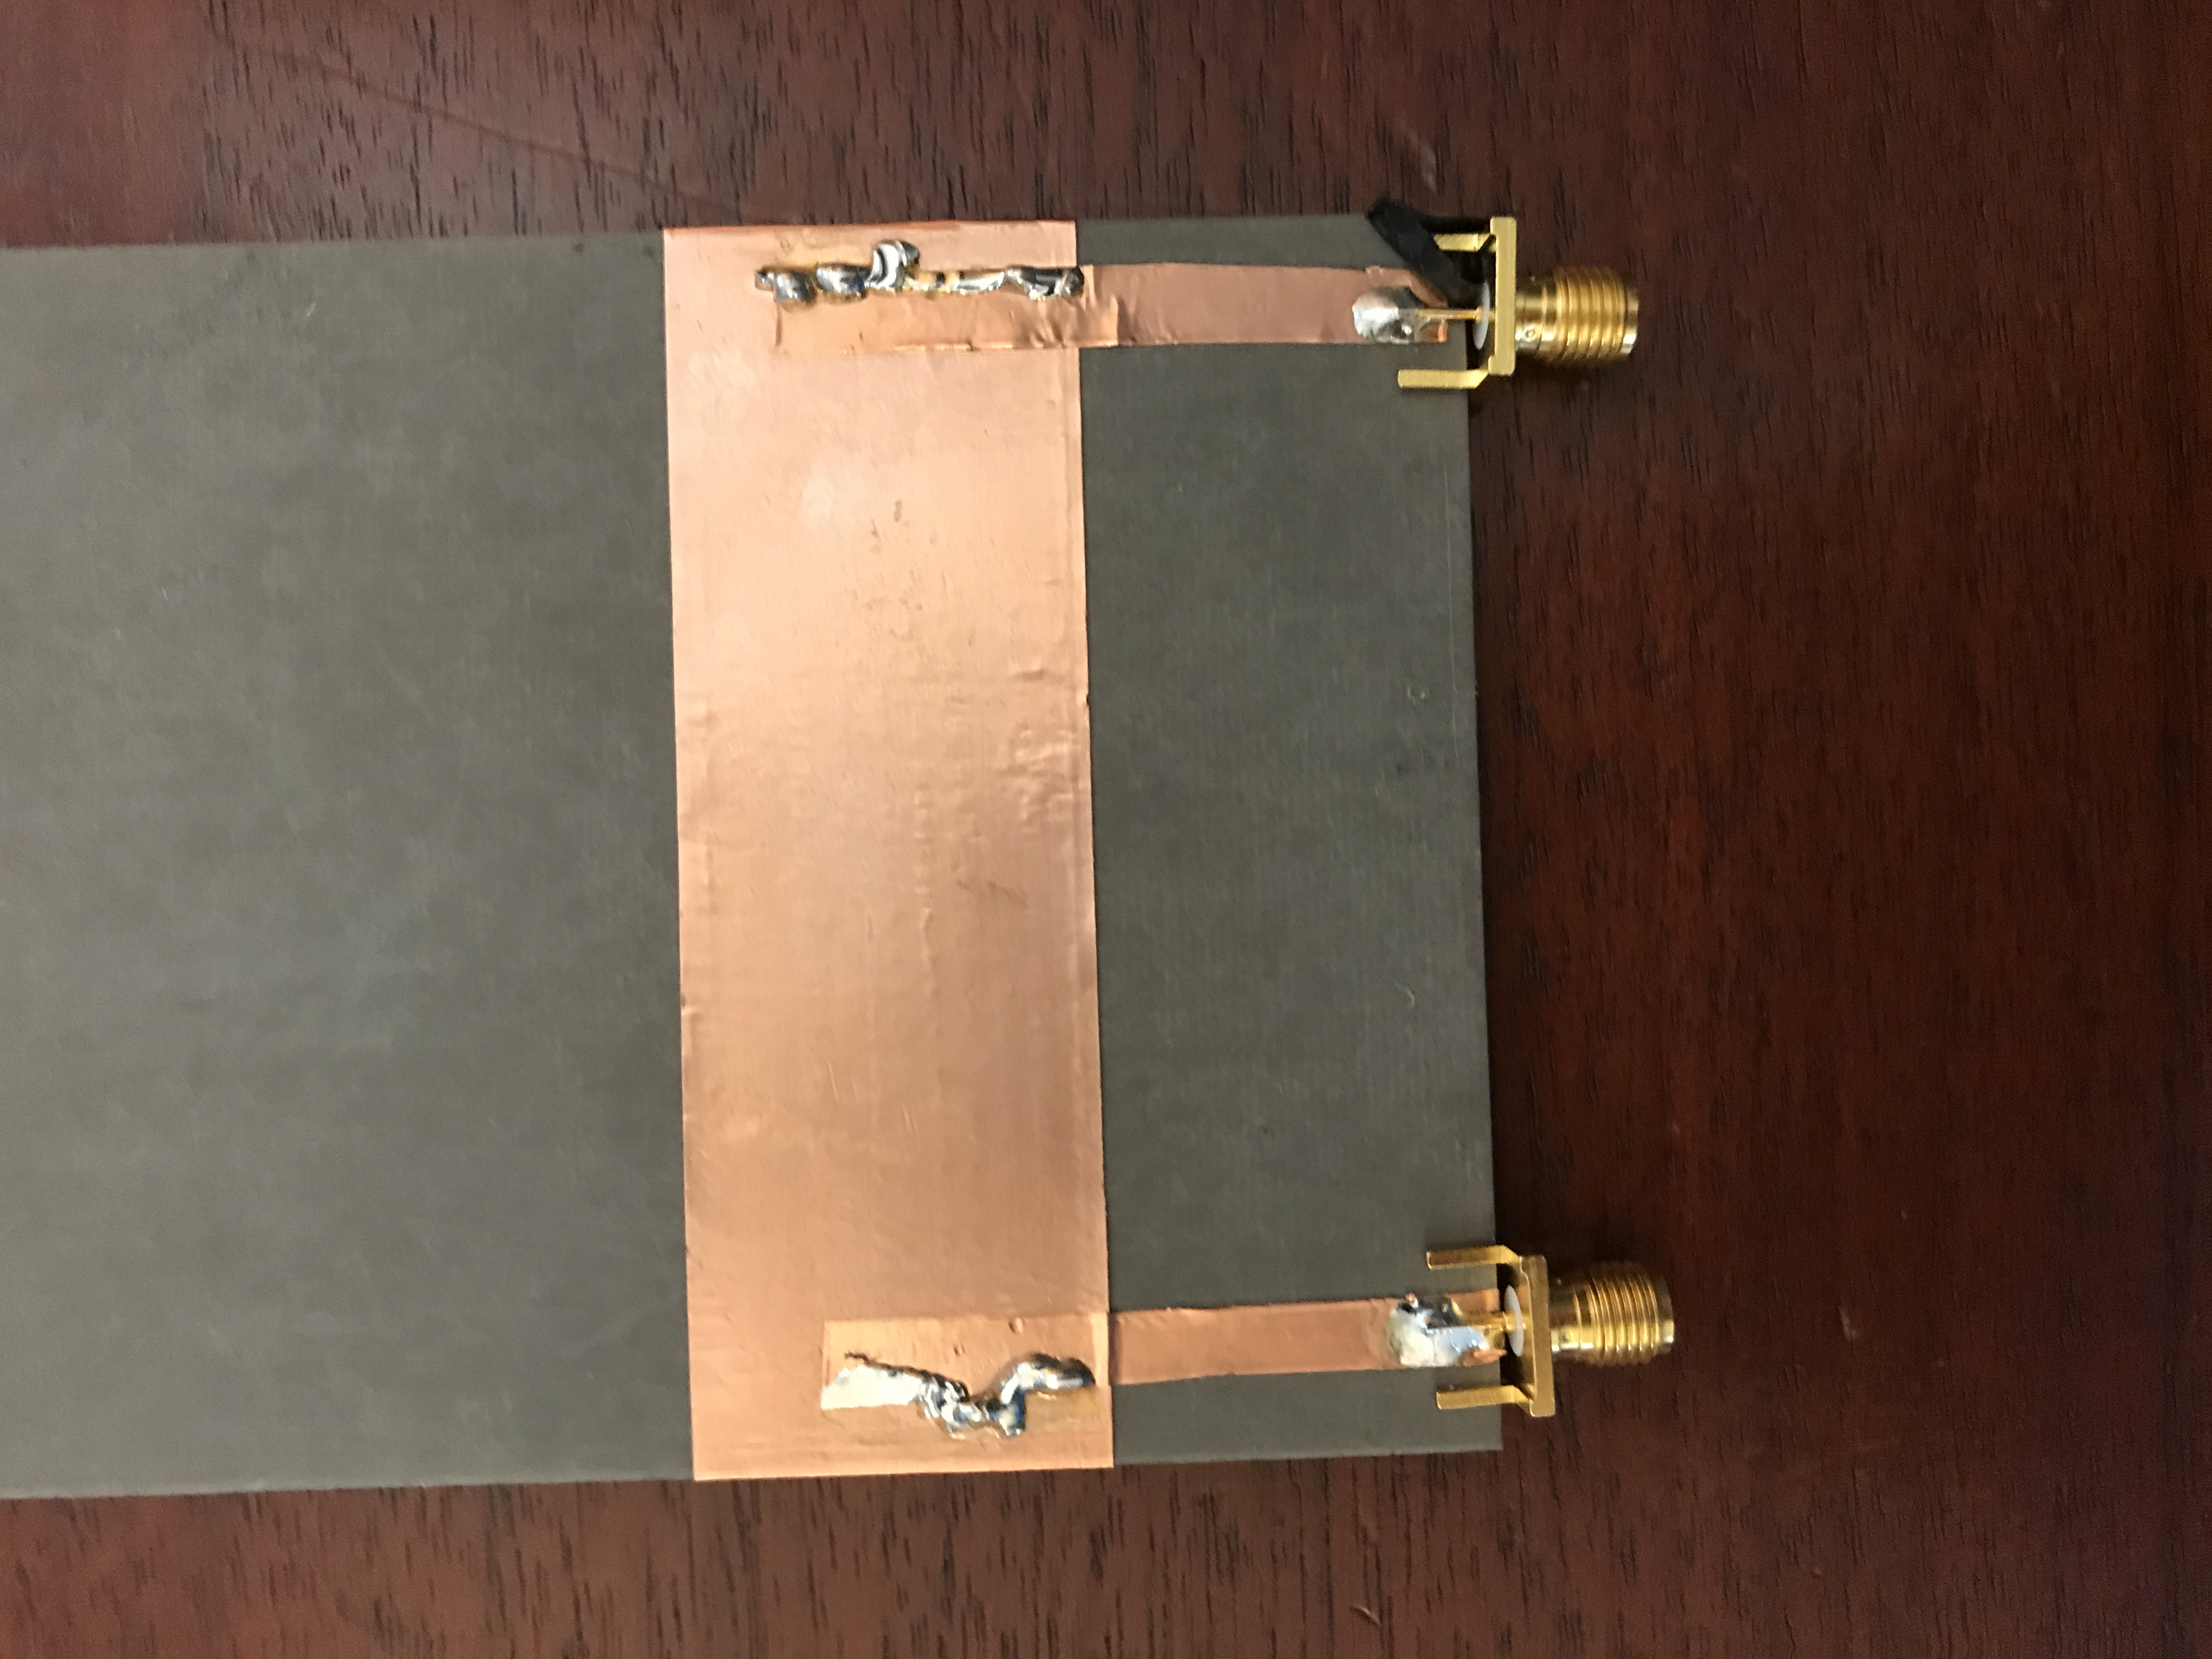
\includegraphics[width=0.8\textwidth, angle = 270]{filter1}
%     \caption{Original width half-wave resonator filter}
% \end{figure}
% \clearpage
\subsection{Short-short 2.4 GHz resonator}
In order to build a filter aimed at our radar's working frequency, we had to design and build a filter that would work at around 2.4 GHz. In order to do so, we used: \(D=\frac{m\cdot\lambda_n}{2}\),\(\lambda_n=\frac{\lambda_0}{n}\), \(m=1\),\(\epsilon_r=2.33\), and \(\mu_r=1\). This calulation resulted in a desired length of \(D=0.0409m\).

% After cutting the substrate boards at the calculated dimensions, we had the following filter:
% \begin{figure}[H]
%     \centering
%     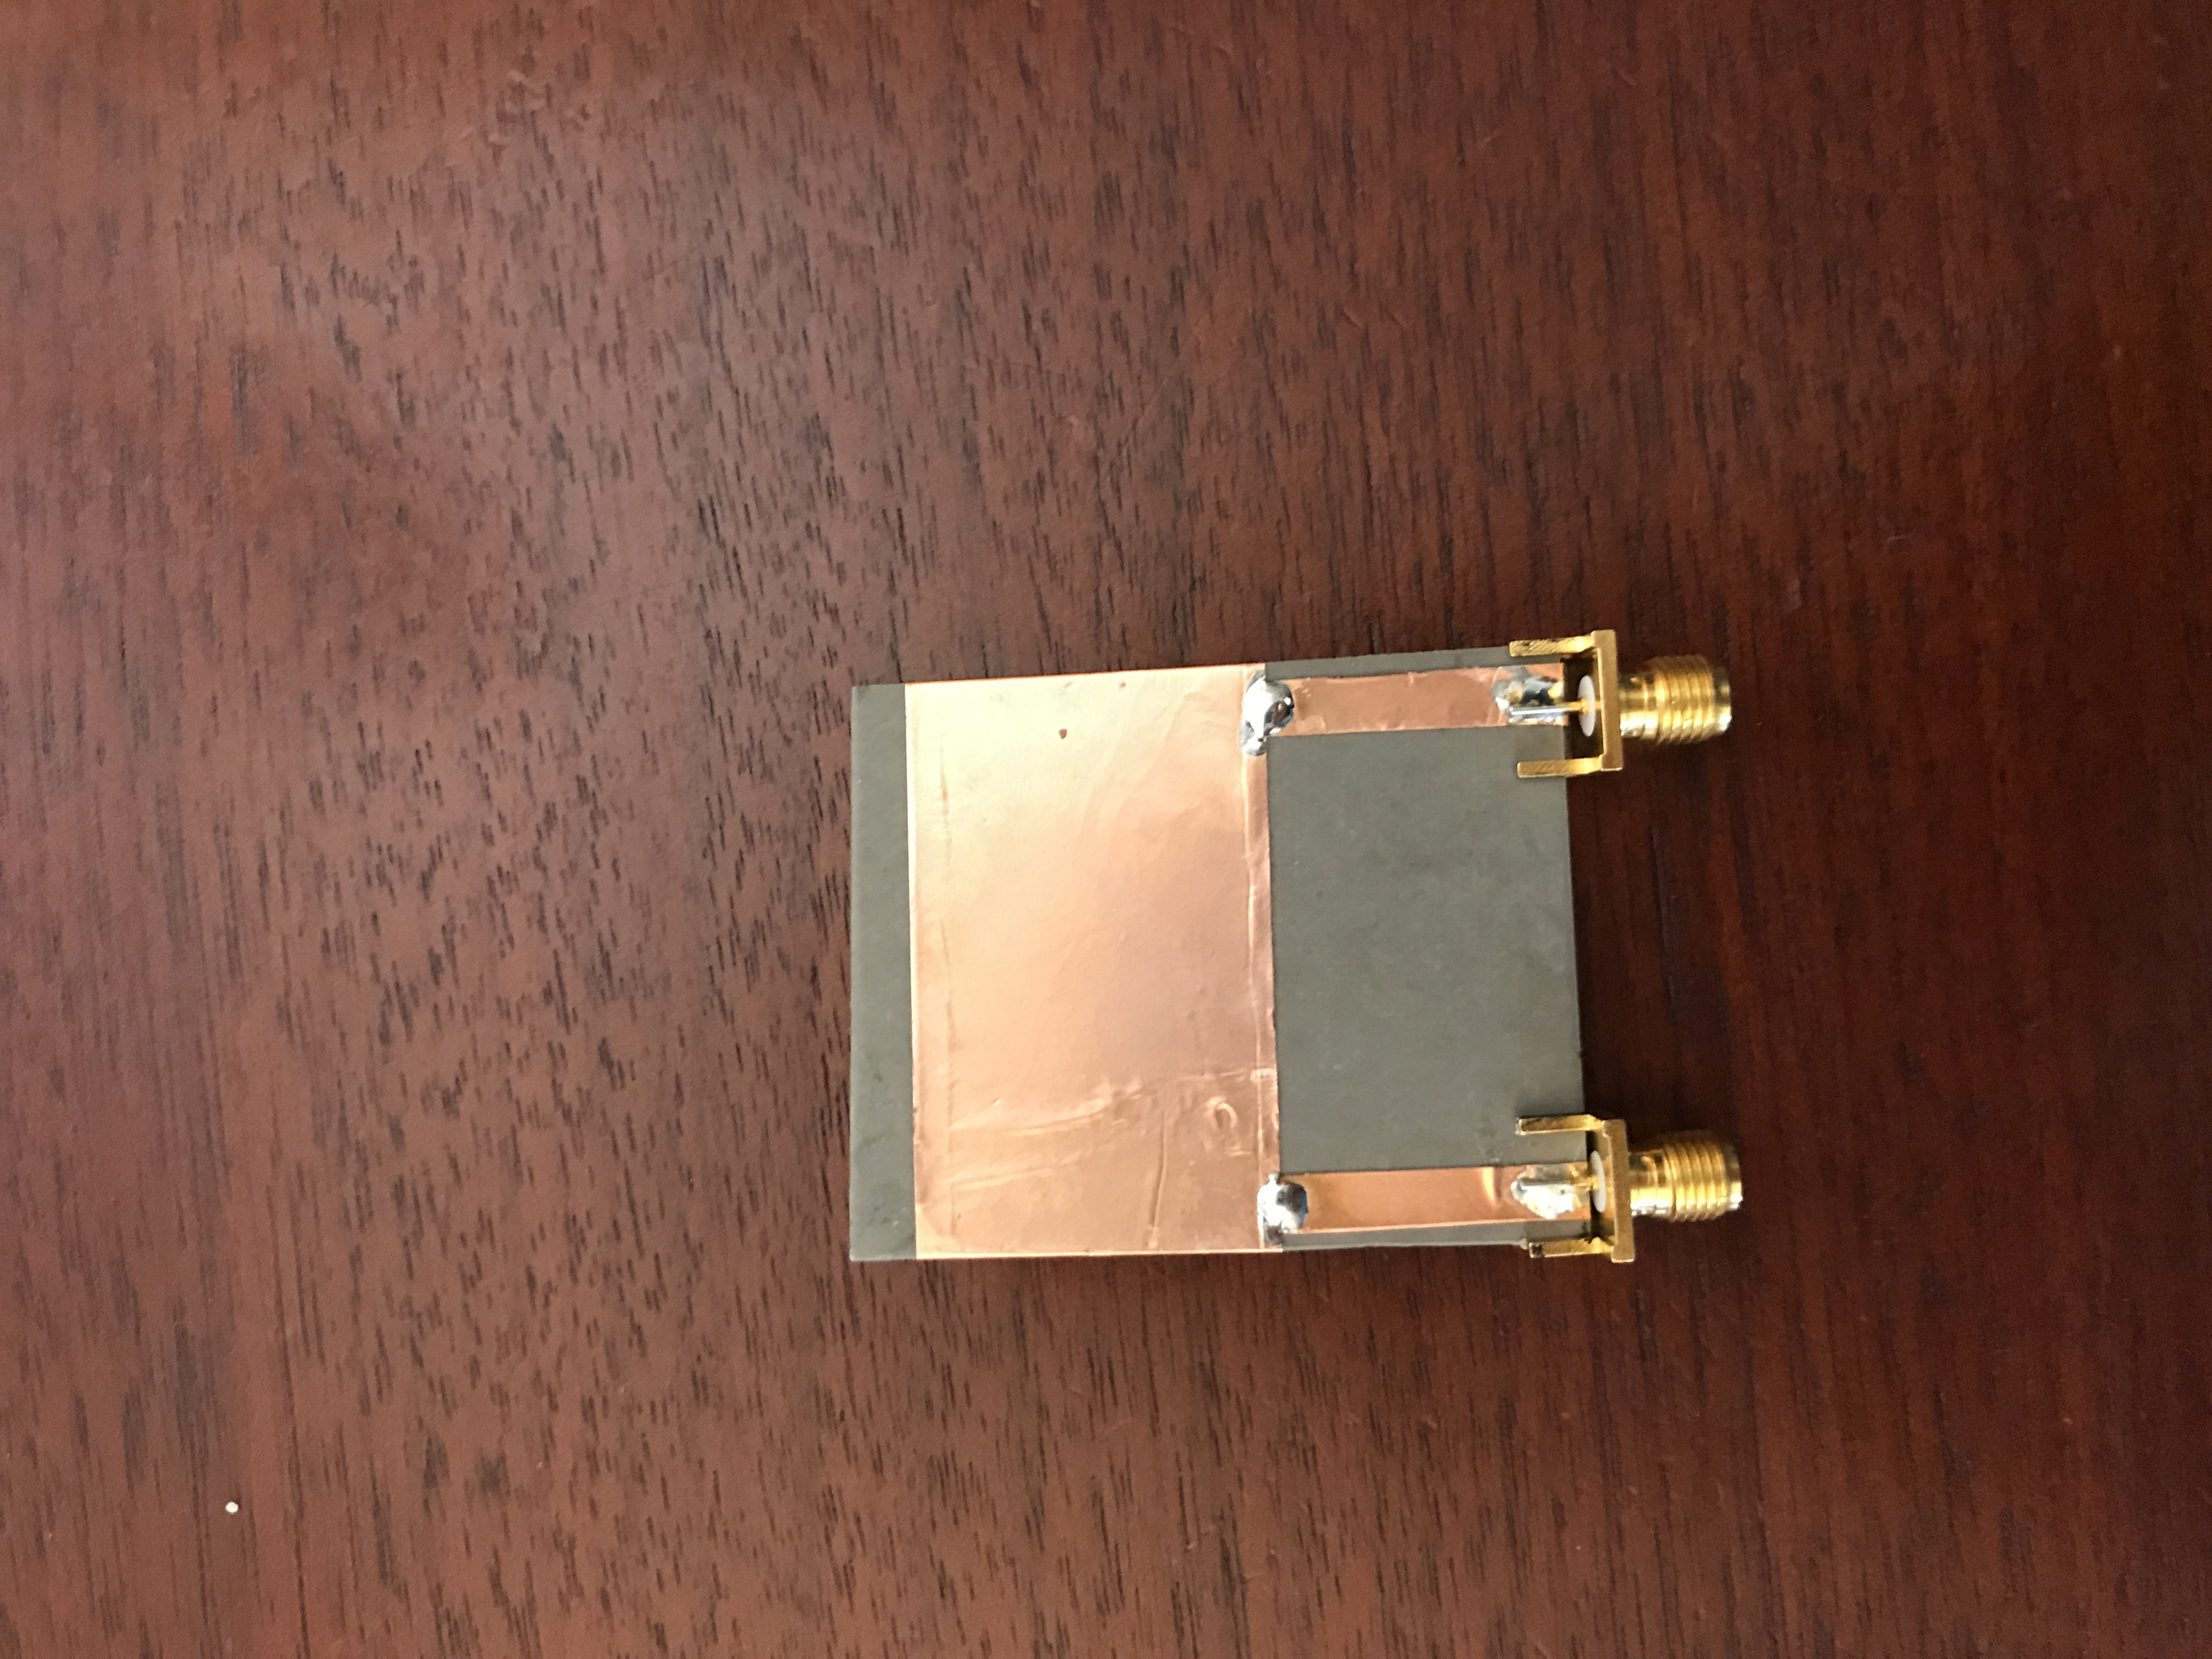
\includegraphics[width=0.8\textwidth, angle = 270]{filter2}
%     \caption{2.4GHz half-wave resonator filter}
% \end{figure}

\subsection{Single stub band-stop filter}
In order in make a band-stop filter, we decided to make a single \(\frac{\lambda}{4}\) stub on a \(50 \Omega\) line. That is designed to transform the open at the end of the stub to a short in parallel with the line which would result in no signal at that frequency. In order to find the correct length, we calculated the wavelength on the substrate, which is \(\lambda=\frac{c/\sqrt(2.33)}{2.4GHz}=0.082m=8.2cm\). That means that our stub has to be \(l=\frac{\lambda}{4}=\frac{8.2}{4}=2.025cm\).
\subsection{multiple stub band-pass filter}
Describe
\section{Results}

\subsection{Short-short half wave resonator}
The short-short 
% \begin{figure}
%     \centering
%     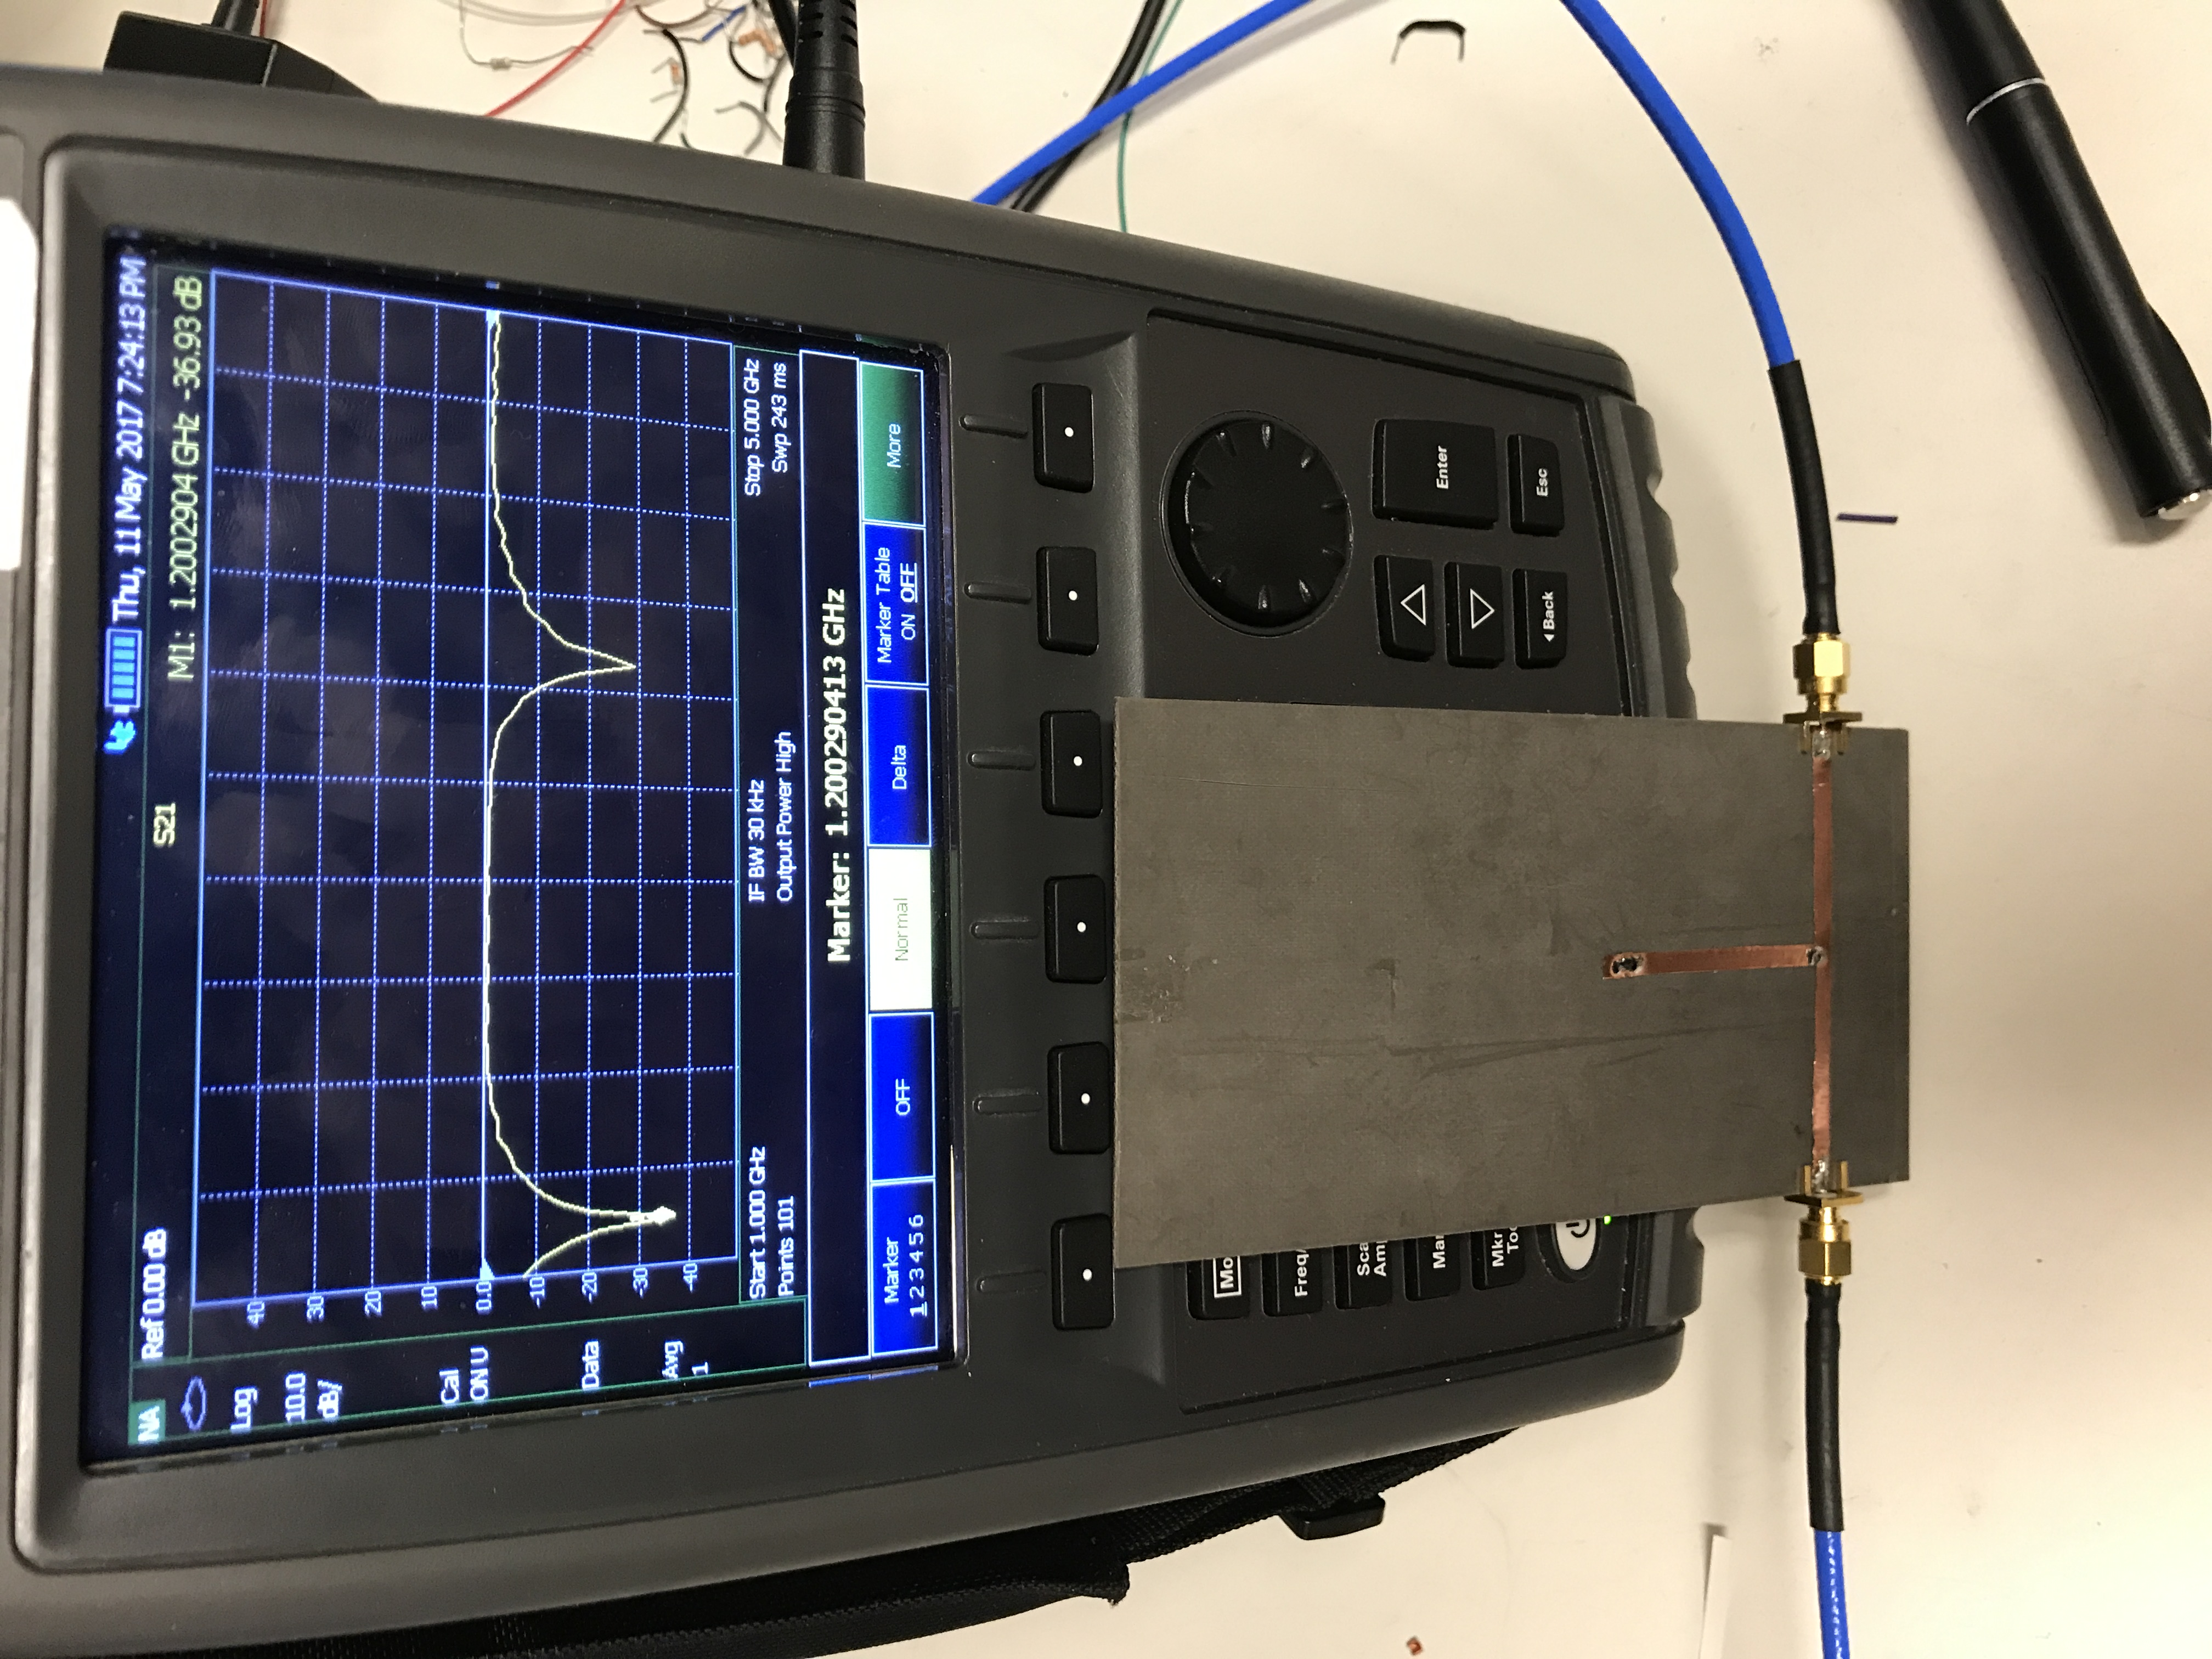
\includegraphics[width=0.8\textwidth, angle=270]{1stub}
%     \caption {single stub measurements}
% \end{figure}
% \subsection{Short-short 2.4 GHz resonator}


\subsection{Single stub band-stop filter}
describe
\subsection{multiple stub band-pass filter}
describes

\section{Conclusion}
describe
\end{document}

